\section{Telegramgruppe \textit{DEMOKRATENCHAT}}
Attila Hildmann hat nicht nur seine eigene Telegram-Gruppe, er ist auch Initiator der Telegram-Gruppe \textit{DEMOKRATENCHAT\autocite{Telegram:demokratenchat3}}, einer Gruppe, in der sich allerlei Verschwörungsideologen alltäglich über Gates, Corona, Merkel, QAnon, Reichsbürger und die Unterdrückung der Menschheit austauschen.\\
Eine Gruppe der Abgehängten, der Schwurbler, der Covidioten, der Benachteiligten ist das, möchte man glauben, eine, in der sich wenig einflussreiche Bürger über ihre Machtlosigkeit echauffieren.

  \textbf{Kein Grund zur Sorge?}\\
  Was, wenn – sagen wir mal – Juristen dort Admins wären? Was, wenn – sagen wir mal – Menschen dort die Regeln überwachen und mitdiskutieren, die als Senior Manager in der Aviation Security einer großen Fluggesellschaft arbeiten?

  \begin{wrapfigure}{r}{0.5\textwidth}\centering  \vspace{-10pt}
    
\includegraphics[width=0.4\textwidth]{images/image--000.jpg}
    \caption{}\label{image:0}
  \end{wrapfigure}
Die Teilnehmerin ``{JS}'' ist \textit{Admin} der Gruppe DEMOKRATENCHAT. Ihr Telegram-Handle ist \emph{@Jusysc}. Sie entscheidet mit, ob ein Beitrag gegen die Regeln verstößt, ob ein Teilnehmer sich daneben benimmt. Sie kann Beiträge löschen und Teilnehmer blockieren (siehe \cref{image:0,image:1}).\\

Als Admin einer Gruppe identifiziert man sich mit den Inhalten der
Gruppe, die man betreut. Man verinnerlicht sie (siehe \cref{image:3}).
\begin{figure}
  \subfloat[Profil von JS]{
    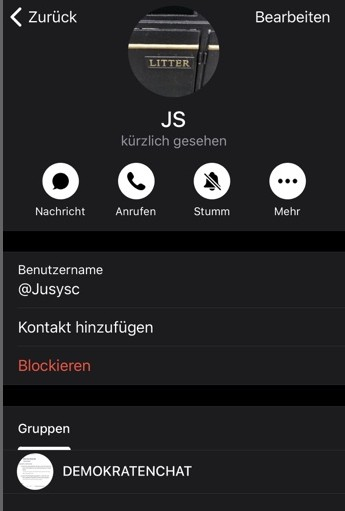
\includegraphics[width=0.3\textwidth]{images/image--001.jpg}
    \label{image:1}
  }
  \subfloat[]{
    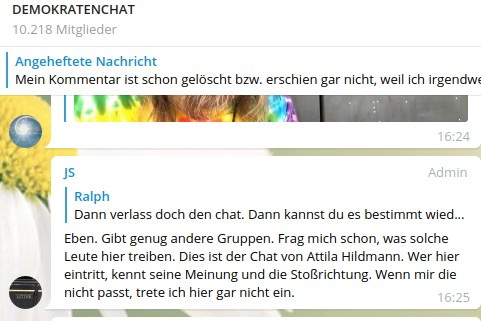
\includegraphics[width=.7\textwidth]{images/image--003.jpg}
    \label{image:3}
  }
  \caption{}
\end{figure}

\begin{wrapfigure}{r}{0.5\textwidth}\centering  \vspace{-20pt}
  \subfloat[]{
    
\includegraphics[width=0.4\textwidth]{images/image--002.jpg}
    \label{image:2}
  }\par
  \subfloat[]{
    
\includegraphics[width=0.4\textwidth]{images/image--006.png}
    \label{image:6}
  }\vspace{-10pt}\caption{}\vspace{-10pt}
\end{wrapfigure}
Und man schreibt ggf. die „Chatregeln“ (siehe \cref{image:2}).


Diese Chatregeln kann in der Telegram-Gruppe jeder herunterladen. Auf die Chatregeln.docx wird von allen Admins der Gruppe immer wieder Bezug genommen. Diese Chatregeln werden immer wieder weitergeleitet \autocite{Telegram:demokratenchat3:regeln}. Sie sind wichtig. Es ist also anzunehmen, dass derjenige, der die Chatregeln erstellt hat, ebenfalls \dots nun \dots vielleicht ein bisschen wichtig ist. Auf jeden Fall steht er in Kontakt mit Attila Hildmann, denn er ist derjenige, der die Admins einsetzt.

  % \begin{wrapfigure}{r}{0.5\textwidth}\centering  \vspace{-10pt}
  %   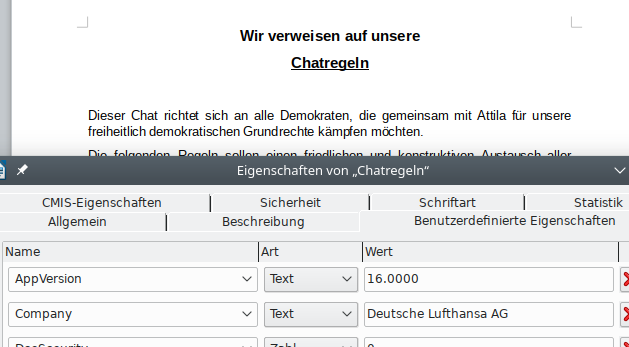
\includegraphics[width=0.4\textwidth]{images/image--004.png}
  %   \caption{}\label{image:4}
  % \end{wrapfigure}
Anonymous Aktivisten sind von Hause aus neugierig. Sie wollen wissen, wer sich hinter dem Kürzel JS versteckt. Und wenn dann ein Word-Dokument verfügbar ist, schauen sie in die Metadaten, denn oft genug findet sich ein hier ein Hinweis. So auch hier, bei „Erstellt“ und „Geändert“ (siehe \cref{image:6}).\\

Jutta Schell hat die Chatregeln geschrieben.\\

Prima. Aber es findet sich noch mehr. Jutta Schell benutzt eine Software, bei der als Firma die Deutsche Lufthansa AG hinterlegt ist (siehe \cref{image:4,image:5}). Damit hat sie am 29.05.2020 die Chatregeln für den DEMOKRATENCHAT geschrieben, dem Chat von Attila Hildmann. Jenem Attila Hildmann, der wegen seiner kruden Verschwörungstheorien in den Medien ist \autocite{3}\autocite{4}\autocite{5}\autocite{6}\autocite{7}.
Sie entscheidet als Admin über Wohl und Wehe von Inhalt und Mitgliedern der Gruppe und bestimmt die Regeln.
\begin{figure}\centering
  \subfloat[]{
    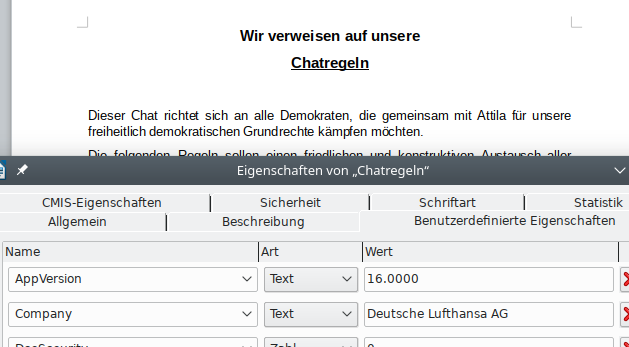
\includegraphics[width=0.6\textwidth]{images/image--004.png}
    \label{image:4}
  }
  \subfloat[]{
    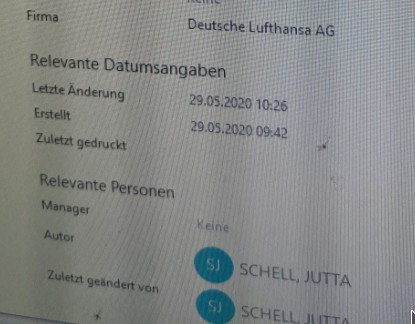
\includegraphics[width=.4\textwidth]{images/image--005.jpg}
    \label{image:5}
  }
  \caption{}
\end{figure}

\newpage
